 \documentclass[12pt,letterpaper, onecolumn]{exam}
\usepackage{amsmath}
\usepackage{amssymb}
\usepackage{amsthm}
\usepackage{graphicx}
\usepackage{mathrsfs}
\usepackage{xcolor}
\usepackage[lmargin=71pt, tmargin=1.2in]{geometry}  %For centering solution box
\usepackage[english]{babel}
\newtheorem{theorem}{Theorem}
\newtheorem{lemma}[theorem]{Lemma}
\usepackage{accents}
\newcommand{\ubar}[1]{\underaccent{\bar}{#1}}
\newcommand{\bs}[1]{\boldsymbol{#1}}
\newcommand{\bm}[1]{\mathbf{#1}}
\newcommand{\der}[2]{\frac{d #1}{d#2}}
\newcommand{\pder}[3]{\frac{\delta^{#3} #1}{\delta^{#3}#2}}
\newcommand{\rs}{$X_1, ..., X_n$}
\newcommand{\nsum}{\sum_{i=1}^n}
\newcommand{\nprod}{\prod_{i=1}^n}
\newcommand*{\Comb}[2]{{}^{#1}C_{#2}}%
\newcommand{\ifc}{\textrm{ if }}
\newcommand{\real}{\mathbb{R}}
\newcommand{\nat}{\mathbb{N}}
\newcommand{\power}{\mathcal{P}}
\newcommand{\rational}{\mathbb{Q}}
\newcommand{\cutelim}{\lim\limits_{n\to\infty}}
\newcommand{\cutesum}[1]{\sum_{#1 = 0}^{\infty}}


% \chead{\hline} % Un-comment to draw line below header
\thispagestyle{empty}   %For removing header/footer from page 1

\begin{document}

\begingroup  
    \centering
    \LARGE STAT 6410\\
    \LARGE Homework 1 \\[0.5em]
    \large Sarah Kilgard\par
\endgroup
\rule{\textwidth}{0.4pt}
\pointsdroppedatright   %Self-explanatory
\printanswers
\renewcommand{\solutiontitle}{\noindent\textbf{Ans:}\enspace}   %Replace "Ans:" with starting keyword in solution box

\begin{questions}
%%%%%%%%%%% Question 1 %%%%%%%%%%%%%%%%%%%%    

    \question A.3 Let $I=[0,1]$, $\Omega=\real$ and for $\alpha\in \real$, $A_\alpha =(\alpha-1,\alpha+1)$, the open
interval $\{x : \alpha - 1 < x < \alpha + 1\}$.
\begin{itemize}
\item[(a)] Show that $\cup_{\alpha\in I} A_\alpha = (-1, 2)$ and $\cap_{\alpha\in I} A_\alpha = (0, 1)$.
\item[(b)] Suppose $J = \{x : x \in I,x \textrm{ is rational}\}$. Find $\cup_{x\in J}A_x$ and $\cap_{ x\in J} A_x$.
\end{itemize}
    \begin{solution}
    (a) 
    \begin{proof}
        $A_0 = (-1, 1)$ and $A_1 = (0, 2)$. Thus, $A_0 \cup A_1 = (-1, 2).$

        \textbf{Part 1:} WTS $\cup_{\alpha \in I} A_\alpha \subset A_0 \cup A_1$.

        Let $x \in \cup_{\alpha \in I} A_\alpha$ be given. \\
        Thus, $\exists \: \beta \in [0,1]$ s.t. $x \in A_\beta$. 
        \\ If this $\beta = 1$, $x \in A_1$.

        If this $\beta \neq 1$:
        Since $\beta - 1$ can be at most 0 and $\beta + 1$ can be at least 1, we know that $0 \in A_\beta$.
        If $x \in (0, \beta + 1$), $x \in (0, 2) = A_1$ because $(0, \beta + 1) \subset (0, 2)$. 
        If $x \in (\beta - 1, 0)$, $x \in (-1, 1) = A_0$ because $(\beta - 1, 0) \subset (-1, 1)$. 

        Thus, $x \in A_0 \cup A_1$. \\ $
        \therefore \: \cup_{\alpha \in I} A_\alpha \subset A_0 \cup A_1$

        \textbf{Part 2:} WTS $A_0 \cup A_1 \subset \cup_{\alpha \in I} A_\alpha $. \\
        This is trivially true

        Thus, $\cup_{\alpha\in I} A_\alpha = A_0 \cup A_1 = (-1, 2)$

        \begin{proof}
            $A_0 = (-1, 1)$ and $A_1 = (0, 2)$. Thus, $A_0 \cap A_1 = (0, 1).$

            \textbf{Part 1:} WTS   $\cap_{\alpha\in I} A_\alpha \subset  A_0 \cap A_1$

            Let $x \in \cap_{\alpha\in I} A_\alpha$ be given. 

            Since, $\max_{\alpha \in I} (\inf (A_\alpha)) = \inf(A_1) = 0$ and similarly, $\min_{\alpha \in I} (\sup (A_\alpha)) = \sup(A_0) = 1$.

            Thus, $0 \leq x \leq 1$. Therefore, $x \in (0, 1) = A_0 \cap A_1$

            \textbf{Part 2:} WTS   $A_0 \cap A_1 \subset \cap_{\alpha\in I} A_\alpha$ \\ This is trivially true. 

            Thus, $\cap_{\alpha\in I} A_\alpha = A_0 \cap A_1 = (0, 1)$

        (b) 

        \textbf{Part 1:}
        Since $\rational \subset \real$, it is clear to see that $\cup_{x\in J}A_x \subset \cup_{x\in I}A_x$.

        We know that rational numbers are dense on real numbers. This means that $\forall \: \alpha \in I, \: \exists \: p, q \in \rational \cap I$ s.t. $p < \alpha < q$.

        So, $A_\alpha = (\alpha - 1, \alpha + 1) \subset (p - 1, q + 1) = (p - 1, p+1) \cup (q - 1, q + 1) = A_p \cup A_q \subset \cup_{x \in J} A_x$. 

        Therefore, $\cup_{x \in J} A_x = \cup_{\alpha \in I} A_\alpha = (-1, 2)$

        \textbf{Part 2:}
        Since, $\rational \subset \real$, it is clear to see that $\cap_{\alpha \in I}A_\alpha \subset \cap_{x\in J}A_x$.

        $\cap_{x\in J}A_x \subset A_0 \cap A_1 = (0, 1) = \cap_{\alpha \in I} A_\alpha$.

        Thus, $\cap_{x\in J}A_x = \cap_{\alpha \in I} A_\alpha = (0, 1) $
        \end{proof}
        
    \end{proof}
    \end{solution}

    

%%%%%%%%%%% Question 2 %%%%%%%%%%%%%%%%%%%%    
    \question A.5 Show that $X \equiv \{0,1\}^\nat$, the set of all sequences $\{\omega_i\}_{i\in \nat}$ where each
$\omega_i \in \{0,1\}$, is \textit{uncountable}. Conclude that $\power(\nat)$ is uncountable.
    \begin{solution}
    \begin{proof}
        $(0, 1)$ is an uncountable set. 
        
        If $X$ is uncountable, there must be a one-to-one function, $f: (0, 1) \to X = \{0, 1\}^{\nat}$, that maps from $(0, 1)$ to $X$.

        Suppose we think of elements, $x$, in $X$ as digits of a base 2 number. For instance, $x = (1, 1, 0, 0, ...)$ are the 1st, 2nd, 3rd, ... digits of number in base 2. ...0000011. This would be 3 in base 10. 

        Here is a verbal description of $f: (0, 1) \to X$:
        \begin{itemize}
            \item[i.] Start with an element of (0, 1). Let's call it $a$.
            \item[ii.] Convert to a natural number, $a^*$, where the 10th place in $a$ is the ones place in $a^*$, the 100th place in $a$ is the tens place in $a^*$, the 1000th place in $a$ is the hundreds place in $a^*$ and so forth. For instance, if $a = 0.9200000...$, $a^* = 29$
            \item[iii.] Convert to $a^*$ to base 2. For instance if $a^* = 29$, it is ...00000010100 in base 10. 
            \item[iv.] Now, we can bring this into $\{0, 1\}^\nat$, where the first digit of the binary version of $a^*$ is the first element in the vector in $X$, the second digit in the binary version of $a^*$ is the 2nd element in the vector of $X$, and so forth. For example, 10100 would be $\{0, 0, 1, 0, 1, 0, 0, ...\}$.
        \end{itemize}
    Conversion from base 10 to base 2 is inherently one-to-one and onto. Each element in $a \in (0,1)$ can uniquely be transformed to a natural number (base 10) as described in (ii), and each natural number can be uniquely transformed to a base 2 number as described in (iii), which can be vectorized uniquely as described in (vi). 

    Thus, $f:(0,1) \to X$ is one-to-one.

    Thus, $|X| = |(0, 1)|$, and $X$ is uncountable. 

    Now we can define a one-to-one (and onto) mapping between them, $g: \power(\nat) \to \{0, 1\}^\nat$:

    For all $Z \in \power(\nat)$, $g(Z) = \{x_i\}_{i \in \nat}$, where $x_i = \begin{cases}
        1 \ifc i \in Z \\
        0 \ifc i \notin Z
    \end{cases}$

    Thus, we can say that $|X| = |\power(\nat)|$. Thus $\power(\nat)$ is uncountable. 
    \end{proof}
    \end{solution}

%%%%%%%%%%% Question 3 %%%%%%%%%%%%%%%%%%%%    
    \question A.9 Apply the principle of induction to establish the following:
    \begin{itemize}
    \item[(a)] For each $n \in \nat$, $\sum_{j=1}^n j^2 = \frac{n(n+1)(2n+1)}{6}$
    \item[(b)] For each $n \in \nat$, $x_1,x_2,...,x_k \in \real$,
\begin{itemize}
    \item[(i)] (\textit{The binomial formula}). $(x_1 +x_2 )^n = \sum_{r=0}^n\binom{n}{r}x_1^rx_2^{n-r}$
    \item[(ii)] (\textit{The multinomial formula}).
$(x_1 +x_2 +...+x_k )^n = \sum \frac{n!}{r_1!r_2!...r_k!}x_1^{r_1}x_2^{r_2} ...x_k^{r_k}$,
where the summation extends over all $(r_1,r_2,...,r_k)$ such
that $r_i \in \nat$, \\ $0\leq r_i \leq n$, $\sum^k_{r=1}r_i =n$.
\end{itemize}
\end{itemize}
    \begin{solution}
    (a)
    \begin{proof}
    Let $\power(n)$ be the mathematical statement $\sum_{j=1}^n j^2 = \frac{n(n+1)(2n+1)}{6}$.
    
    i) WTS $\power(1)$ is true. \\
    Left Side: $\sum_{j=1}^1 j^2 = 1$ \\
    Right Side: $\frac{1(1+1)(2(1)+1)}{6} = \frac{6}{6} = 1$
    Since the left side = right side, $\power(1)$ holds true. 

    ii) WTS that $\power(n)$ is true $ \implies \: \power(n+1)$ is true. \\
    Let $n \in \nat$ be given. Suppose $\power(n)$ is true. \\
    Thus, $\sum_{j=1}^n j^2 = \frac{n(n+1)(2n+1)}{6}$.

    $\sum_{j=1}^{n+1} j^2 = \sum_{j=1}^n j^2 + (n+1)^2 = \frac{n(n+1)(2n+1)}{6} + (n+1)^2 = \frac{2n^3 + 3n^2 + n}{6} + \frac{6n^2 + 12n + 6}{6}$ \\
    $ = \frac{2n^3 + 9n^2 +12n + 6}{6} = \frac{(n+1)((n+1) + 1)(2(n+1)+1)}{6}$

    Thus, $\power(n+1)$ is true. 

    By induction, we can say that $\power(n)$ is true for all $n \in \nat$
    \end{proof}

    (b.i) 
    \begin{proof}
     Let $\power(n)$ be the mathematical statement 
    $(x_1 +x_2 )^n = \sum_{r=0}^n\binom{n}{r}x_1^rx_2^{n-r}$.
    i) WTS $\power(1)$ is true. \\
        Left Side:  $(x_1 + x_2)^1 = x_1 + x_2$\\
        Right Side: $\sum_{r=0}^1\binom{1}{r}x_1^rx_2^{1-r} = \binom{1}{0}x_1^0x_2^{1-0} + \binom{1}{1}x_1^1x_2^{1-1} = x_1 + x_2$

    Since The LHS = RHS, $\power(1)$ is true.

    ii) WTS that $\power(n)$ is true $ \implies \: \power(n+1)$ is true. \\
    Let $n \in \nat$ be given. Suppose $\power(n)$ is true. \\
    Thus, $(x_1 +x_2 )^n = \sum_{r=0}^n\binom{n}{r}x_1^rx_2^{n-r}$

    \[(x_1 + x_2)^{n+1} = (x_1 + x_2)^{n}(x_1 + x_2) = \sum_{r=0}^n\binom{n}{r}x_1^rx_2^{n-r} (x_1 + x_2)\]
    \[= x_1\sum_{r=0}^n\binom{n}{r}x_1^rx_2^{n-r} + x_2 \sum_{r=0}^n\binom{n}{r}x_1^rx_2^{n-r} = \sum_{r=0}^n\binom{n}{r}x_1^{r+1}x_2^{n-r} + \sum_{r=0}^n\binom{n}{r}x_1^rx_2^{n+1-r}\]
    \[=\binom{n}{n}x_1^{n+1} + \sum_{r=0}^{n-1}\binom{n}{r}x_1^{r+1} x_2^{n-r} + \binom{n}{0}x_2^{n+1} + \sum_{r=1}^{n}\binom{n}{r}x_1^{r} x_2^{n+-r}\] 
    \[=x_1^{n+1} + \sum_{r=1}^{n}\binom{n}{r-1}x_1^{r} x_2^{n+1-r} + x_2^{n+1} + \sum_{r=1}^{n}\binom{n}{r}x_1^{r} x_2^{n+1-r}\]
    \[= \sum_{r=0}^{0}\binom{n+1}{r}x_1^rx_2^{n+1-r} \sum_{r=n+1}^{n+1}\binom{n+1}{r}x_1^rx_2^{n+1-r} + \sum_{r=1}^{n}\binom{n+1}{r}x_1^{r} x_2^{n+1-r}\]
    By Pascal's Law
    \[= \sum_{r=0}^{n+1} \binom{n+1}{r}x_1^rx_2^{n+1-r}\]

    Thus, $\power(n)$ is true $\implies \: \power(n+1)$. Thus, by induction: \\
    For each $n \in \nat$, $x_1,x_2,...,x_k \in \real$, \\
    $(x_1 +x_2 +...+x_k )^n = \sum \frac{n!}{r_1!r_2!...r_k!}x_1^{r_1}x_2^{r_2} ...x_k^{r_k}$, \\
where the summation extends over all $(r_1,r_2,...,r_k)$ such
that $r_i \in \nat$, \\ $0\leq r_i \leq n$, $\sum^k_{r=1}r_i =n$.
    \end{proof}

    (b.ii) 
    \begin{proof}
    Let $\power(n)$ be the mathematical statement \\ $(x_1 +x_2 +...+x_k )^n = \sum_{} \frac{n!}{r_1!r_2!...r_k!}x_1^{r_1}x_2^{r_2} ...x_k^{r_k}$, where the summation extends over all $(r_1,r_2,...,r_k)$ such that $r_i \in \nat$, $0\leq r_i \leq n$, $\sum^k_{i=1}r_i =n$
    
    i) WTS $\power(1)$ is true. \\
        Left Side:  $(x_1 +x_2 +...+x_k )^1 = x_1 +x_2 +...+x_k$\\
            $0 \leq r_i \leq 1, \: \sum_{i=1}^k r_i = 1$ \\
            Since $r_i \in \nat$, and $\sum_{i=1}^kr_i$, we know that exactly one $r_i =1$ in any $(r_1, r_2, ..., r_k)$. \\
        Right Side: $\sum \frac{1!}{r_1!r_2!...r_k!}x_1^{r_1}x_2^{r_2} ...x_k^{r_k} = \frac{1!}{1!0!...0!}x_1^1x_2^0...x_k^0 + \frac{1!}{0!1!...0!}x_1^0x_2^1...x_k^0 + ... + \frac{1!}{0!0!...1!}x_1^0x_2^0...x_k^1 = x_1 + x_2 + ... + x_k$

        Since The LHS = RHS, $\power(1)$ is true. 
        

    ii) WTS that $\power(n)$ is true $ \implies \: \power(n+1)$ is true. \\
    Let $n \in \nat$ be given. Suppose $\power(n)$ is true. \\

    Thus, \\
    $(x_1 +x_2 +...+x_k )^n = \sum_{\sum r_i = n} \frac{n!}{r_1!r_2!...r_k!}x_1^{r_1}x_2^{r_2} ...x_k^{r_k}$, where the summation extends over all $(r_1,r_2,...,r_k)$ such that $r_i \in \nat$, $0\leq r_i \leq n$, $\sum^k_{i=1}r_i =n$

    $x_1 + x_2 + ... + x_k)^{n+1} = (x_1 + x_2 + ... + x_k)^n (x_1 + x_2 + ... + x_k) \\ = \underset{\sum r_i = n}{\sum} \frac{n!}{r_1!r_2!...r_k!}x_1^{r_1+1}x_2^{r_2} ...x_k^{r_k} + \underset{\sum r_i = n}{\sum} \frac{n!}{r_1!r_2!...r_k!}x_1^{r_1}x_2^{r_2+1} ...x_k^{r_k} + ... \\ + \underset{\sum r_i = n}{\sum} \frac{n!}{r_1!r_2!...r_k!}x_1^{r_1}x_2^{r_2} ...x_k^{r_k+1}\\
    = \sum_{\sum r_i = n+1}\frac{n!}{(r_1-1)!r_2!...r_k!}x_1^{r_1}x_2^{r_2} ...x_k^{r_k} + \sum_{\sum r_i = n+1}\frac{n!}{r_1!(r_2-1)!...r_k!}x_1^{r_1}x_2^{r_2} ...x_k^{r_k} + ... + \sum_{\sum r_i = n+1}\frac{n!}{(r_1)!r_2!...(r_k-1)!}x_1^{r_1}x_2^{r_2} ...x_k^{r_k}\\
    = \underset{\sum r_i = n+1}{\sum} \frac{(n+1)!}{r_1!r_2!...r_k!}x_1^{r_1}x_2^{r_2} ...x_k^{r_k}$ 

    By the generalization of Pascal's Law.
    
    Thus, $\power(n)$ is true $\implies \: \power(n+1)$. Thus, by induction: \\
    $(x_1 +x_2 +...+x_k )^n = \sum \frac{n!}{r_1!r_2!...r_k!}x_1^{r_1}x_2^{r_2} ...x_k^{r_k}$,
where the summation extends over all $(r_1,r_2,...,r_k)$ such
that $r_i \in \nat$, \\ $0\leq r_i \leq n$, $\sum^k_{r=1}r_i =n$.
    \end{proof}
    \end{solution}

%%%%%%%%%%% Question 4 %%%%%%%%%%%%%%%%%%%%    
    \question A.11 Show that the set $A=\{r:r \in \rational,r^2 <2\}$ is bounded above in $\rational$ but has no l.u.b. in $\rational$.
    \begin{solution}

    \begin{proof}
        Let $x \in A$ be given. Thus, $x^2 < 2$. \\
        $4 \in \rational$, and $4^2 = 16 > 2$. Thus, $x < 4$. \\
        By the definition of an upper bound, 4 is an upper bound of $A$. 
    \end{proof}
    \begin{proof}
        Suppose to the contrary that $sup(A) = M$. Thus, $x \in A \: \implies \: x \leq M$, and $K < sup(A) \: \implies \: \exists \: x \in A \: s.t. \: x \leq M$ and that if $K < M$, $\exists \: x^* \in A \: s.t. \: K < x^*$.\\

        We know that $M < \sqrt{2}$. $M \neq \sqrt{2}$, since $\sqrt{2}$ is irrational. 

        $M, \sqrt{2} \in \real$, so by a corollary of the AOE, there exists a $b \in \rational$ such that $M < b < \sqrt{2}$. 

        There is a contradiction here, because $b < \sqrt{2} \: \implies \: b^2 < 2 \implies b \in A$. But, if M is the supremum of A this cannot be the case. 

        Thus, A has no l.u.b. in $\rational$.
    \end{proof}
    \end{solution}


%%%%%%%%%%% Question 5 %%%%%%%%%%%%%%%%%%%%    
    \question A.12 Show that for any two sequences $\{x_n\}{n\geq 1}$, $\{y_n\}_{n \geq 1} \subset \real$,
\[ \underline{\lim}_{n\to\infty}x_n + \underline{\lim}_{n\to\infty} y_n \leq \underline{\lim}_{n\to\infty}(x_n + y_n) \leq \overline{\lim}_{n \to \infty}(x_n + y_n) \leq \overline{\lim}_{n\to\infty} x_n + \overline{\lim}_{n\to\infty} y_n\]
    \begin{solution}
        \begin{proof}
        Based on the definitions of infimums and supremums: \\
        $\inf_{k \geq n} x_n + \inf_{k \geq n}y_n \leq x_n + y_n \leq  \sup_{k \geq n} x_n + \sup_{k \geq n}y_n$. \\ Thus, $\underline{\lim}_{n\to\infty}x_n + \underline{\lim}_{n\to\infty} y_n \leq \overline{\lim}_{n\to\infty} x_n + \overline{\lim}_{n\to\infty} y_n$

        

        It is also clear to see that $\inf_{k \geq n}(x_n + y_n) \leq \sup_{k \geq n}(x_n + y_n)$, which implies that: $\lim_{n\to\infty}\inf_{k \geq n}(x_n + y_n) \leq \lim_{n \to \infty}\sup_{k \geq n}(x_n + y_n)$ $\iff \\\underline{\lim}_{n\to\infty}(x_n + y_n) \leq \overline{\lim}_{n \to \infty}(x_n + y_n)$
        
        Putting this all together, we get: \\ 
        $ \underline{\lim}_{n\to\infty}x_n + \underline{\lim}_{n\to\infty} y_n \leq \underline{\lim}_{n\to\infty}(x_n + y_n) \leq \overline{\lim}_{n \to \infty}(x_n + y_n) \\ \leq \overline{\lim}_{n\to\infty} x_n + \overline{\lim}_{n\to\infty} y_n$
        \end{proof}
    \end{solution}

%%%%%%%%%%% Question 6 %%%%%%%%%%%%%%%%%%%%    
    \question A.17 Find the radius of convergence, $\rho$, for the powers series $A(x) \equiv \sum^\infty_{n=0} a_n x^n$ where 
    \begin{itemize}
    \item[(a)] $a_n= \frac{n}{n+1}$, $n\geq0$.
    \item[(b)] $a_n =n^p$, $n\geq0$, $p\in \real$.
    \item[(c)] $a_n = \frac{1}{n!}$, $n \geq 0$ (where $0! = 1$).
    \end{itemize}
    \begin{solution}
    Suppose we have a sequence B of positive numbers. If $\log(B_n) \to b$ as $n \to \infty$, then $B \to e^b$ as $n \to \infty$. This fact will be used in the rest of the problem. 

    Additionally, if $\lim\limits_{n\to\infty}a_n$ exists, $\lim\limits_{n\to\infty}a_n =\lim\limits_{n\to\infty}\textrm{sup}a_n  = \lim\limits_{n\to\infty}\textrm{inf}a_n$ if $a_n$ is an sequence of real numbers. This fact will also be used in the next parts. 
    \begin{itemize}
        \item[(a)]
        $\rho = (\lim\limits_{n\to\infty}\textrm{sup}|a_n|^{\tfrac{1}{n}})^{-1} = (\lim\limits_{n\to\infty}\textrm{sup}|\frac{n}{n+1}|^{\tfrac{1}{n}})^{-1} = (\lim\limits_{n\to\infty}\textrm{sup}(\frac{n}{n+1})^{\tfrac{1}{n}})^{-1}$. 

        $\cutelim\log((\frac{n}{n+1})^{\tfrac{1}{n}}) = \cutelim\frac{1}{n}\log(\frac{n}{n+1}) = \cutelim \frac{\log(n) - \log(n+1)}{n}$ \\
        By L'Hopital's rule, $= \cutelim \frac{\tfrac{1}{n} - \frac{1}{n+1}}{1} = \cutelim \frac{1}{n^2 + n}$
        By L'H, = 0

        Thus, $\cutelim(\frac{n}{n+1})^\frac{1}{n} = e^0 = 1 \implies \cutelim\textrm{sup}(\frac{n}{n+1})^\frac{1}{n} = 1$

        Thus, $\rho = (1)^{-1} = 1$
        \item[(b)]
        $\rho = (\lim\limits_{n\to\infty}\textrm{sup}|a_n|^{\tfrac{1}{n}})^{-1} = (\lim\limits_{n\to\infty}\textrm{sup}|n^p|^{\tfrac{1}{n}})^{-1} = (\lim\limits_{n\to\infty}\textrm{sup} (n^{\tfrac{p}{n}}))^{-1}$

        $\cutelim \log(n^{p/n}) = \cutelim\frac{p\log(n)}{n}$

        By L'H, $=\cutelim \frac{p}{n} = p \cutelim\frac{1}{n} = 0$.

        Thus, $\cutelim (n^{p/n}) = e^0=1 \implies \cutelim \textrm{sup}(n^{p/n}) = 1$.

        Thus, $\rho = 1^{-1} = 1$
        \item[(c)]
        $\rho = (\lim\limits_{n\to\infty}\textrm{sup}|a_n|^{\tfrac{1}{n}})^{-1} = (\lim\limits_{n\to\infty}\textrm{sup}|\frac{1}{n!}|^{\tfrac{1}{n}})^{-1}$

        We can show that $\cutelim (\frac{1}{n})^{1/n} = 0$ using L'H: \\
         $\cutelim (\frac{1}{n})^{1/n} = \cutelim \frac{1}{n^{1/n}}$ \\
         By L'H, $= \cutelim \frac{0}{\frac{1}{n}n^{1-1/n}} = \cutelim 0 = 0$

         We know that $\frac{1}{n} \geq \frac{1}{n!}$ when $n > 0$. (Since we are looking at the limit as $n \to \infty$, we do not need to concern ourselves with what happens when n = 0). \\
         Thus, $(\frac{1}{n})^{1/n} \geq (\frac{1}{n!})^{1/n}$ when $n > 0$. It is clear to see that $(\frac{1}{n!})^{1/n}$ cannot be less than 0, and since $(\frac{1}{n})^{1/n} \geq (\frac{1}{n!})^{1/n}$, we can assume that $\cutelim (\frac{1}{n!})^{1/n}$ cannot be greater than $\cutelim(\frac{1}{n})^{1/n}$. \\
         Thus, $\cutelim (\frac{1}{n!})^{1/n} = 0$.

         Thus, $\cutelim \textrm{sup}(\frac{1}{n!})^{1/n} = 0 \: \implies \rho = (0)^{-1} = \infty$.

         This means that the radius of convergence diverges to $+ \infty $
    \end{itemize}
    \end{solution}

%%%%%%%%%%% Question 7 %%%%%%%%%%%%%%%%%%%%    
    \question 
    A.18 
    \begin{itemize}
    \item[(a)] Find the Taylor series at $a = 0$ for the function $f(x) = \frac{1}{1-x}$ on $I \equiv (-1,+1)$ and show that it converges to $f(x)$ on $I$.
    \item[(b)] Find the Taylor series of $1+x+x^2$ in $I=(1,3)$, \: centered at $2$.
    \item[(c)] Let
    \[f(x) = \begin{cases}
        e^{-1/x^2} \ifc |x| < 1, \: x \neq 0 \\
        0 \ifc x = 0
    \end{cases}\]
    \begin{itemize}
    \item[(i)] Show that $f$ is infinitely differentiable at $0$ and compute $f^{(j)}$ for all $j \geq 1$
    \item[(ii)] Show that the Taylor series at $a = 0$ converges but not to f on $(-1, 1)$.
    \end{itemize}
    \end{itemize}
    \begin{solution}
    \begin{itemize}
    \item[(a)]
    $f^{(n)}(x) = \frac{n!}{(1-x)^{n+1}}$ \\
    $\sum_{n=0}^\infty \frac{f^{(n)}(a)}{n!}(x-a)^n = \cutesum{n} \frac{1}{n!}\frac{n!}{(1-0)^{n+1}} (x-0)^n = \cutesum{n} x^n$
    This is a geometric series, and it converges when $x \in (-1,1) = I$ to $\frac{1}{1-x}.$
    \item[(b)]
    $f^{(0)}(1) = 1 + 1 + (1)^2 = 3, \: f^{(1)}(1) = 1 + 2(1) = 3, \: f^{(2)}(1) = 2, \\f^{(3)}(1) = 0, f^{(4)}(1) = 0 , ...$
    
    $\cutesum{n}\frac{f^{(n)}(a)}{n!}(x-a)^n = \frac{3}{0!}(x-1)^0 + \frac{3}{1!}(x-1)^1 + \frac{2}{2!}(x-1)^2 + \frac{0}{3!}(x-1)^3 + 0 + ... \\ = 3 + 3x - 1 + x^2 -2x + 1 + 0 + 0 + ... \\ = x^2 - x + 3$ for $x \in I = (1, 3)$

    
    \item[(c)] 
    (i) We know that $g(x) = e^{-x}$ is infinitely differentiable on x, as $g^{(j)}(x) = (-1)^{j}e^{-x}$ for all $j = 1, 2, ...$, and we also know that $h(x) = \frac{1}{x^2} = x^{-2}$ is infinitely differentiable, as $h^{(j)}(x) = (-1)^{j}\frac{j!}{x^{2+j}}$.

    By the chain rule, since both $g(x)$ and $h(x)$ are infinitely differentiable, we know that $f(x) = g(h(x))$ is also infinitely differentiable. And thus, $f^{(j)}(0) = 0$
    
    
    (ii) $f^{n} = 0, \: \forall \: x \in \nat \cup \{0\}$, so $\sum_{n=0}^\infty \frac{f^{(n)}(0)}{n!}(x-0)^n = \cutesum{n} 0 = 0$. Thus, regardless of your choice of $x \in (-1, 1)\cap\{0\}^c,$ the Taylor series will converge to 0, not $f(x) $
    \end{itemize}
    \end{solution}

%%%%%%%%%%% Question 8 %%%%%%%%%%%%%%%%%%%%    
    \question A.24
    \begin{itemize}
\item[(c)] Draw the open unit ball $B_p \equiv
\{x:x\in \real^2, d_p(x,0)<1\}$ in $\real^2$ for $p = 1, 2$ and $\infty$.
\end{itemize}

\begin{figure}[h!]
    \centering
    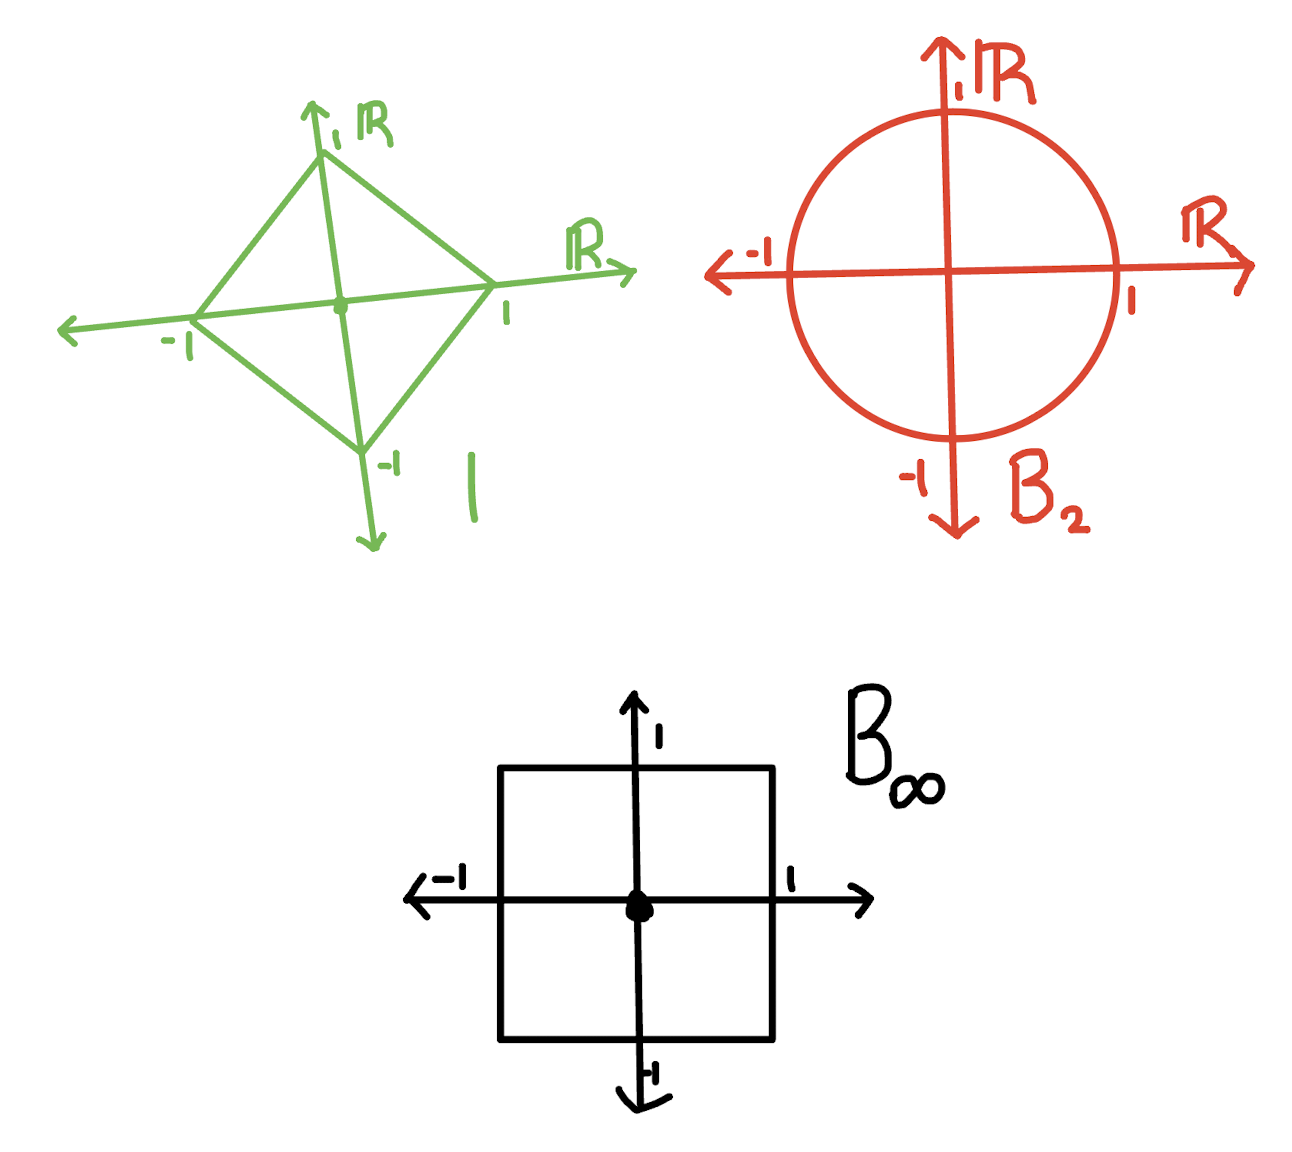
\includegraphics[width=0.5\linewidth]{images/hw1.balls.png}
\end{figure}
The green is $B_1$, the red is $B_2$, and the black is $B_\infty$

\end{questions}
\end{document}